% Created by tikzDevice version 0.12.3.1 on 2021-04-13 14:32:59
% !TEX encoding = UTF-8 Unicode
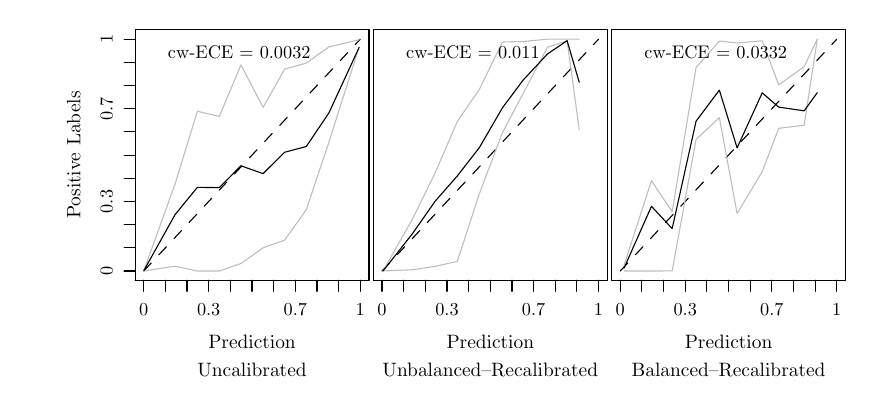
\begin{tikzpicture}[x=1pt,y=1pt]
\definecolor{fillColor}{RGB}{255,255,255}
\path[use as bounding box,fill=fillColor,fill opacity=0.00] (0,0) rectangle (296.31,130.09);
\begin{scope}
\path[clip] (  0.00,  0.00) rectangle (296.31,130.09);
\definecolor{drawColor}{RGB}{0,0,0}

\path[draw=drawColor,line width= 0.4pt,line join=round,line cap=round] ( 38.81, 38.81) --
	(123.32, 38.81) --
	(123.32,129.29) --
	( 38.81,129.29) --
	( 38.81, 38.81);
\end{scope}
\begin{scope}
\path[clip] ( 38.81, 38.81) rectangle (123.32,129.29);
\definecolor{drawColor}{RGB}{0,0,0}

\path[draw=drawColor,line width= 0.4pt,dash pattern=on 4pt off 4pt ,line join=round,line cap=round] ( 41.94, 42.16) --
	(120.19,125.94);
\definecolor{drawColor}{RGB}{190,190,190}

\path[draw=drawColor,line width= 0.4pt,line join=round,line cap=round] ( 41.95, 42.17) --
	( 53.25, 43.90) --
	( 61.32, 42.16) --
	( 69.25, 42.16) --
	( 77.05, 44.86) --
	( 85.07, 50.54) --
	( 92.85, 53.33) --
	(100.69, 64.34) --
	(108.84, 88.71) --
	(119.78,123.05);

\path[draw=drawColor,line width= 0.4pt,line join=round,line cap=round] ( 41.95, 42.23) --
	( 53.25, 73.58) --
	( 61.32, 99.88) --
	( 69.25, 98.01) --
	( 77.05,116.63) --
	( 85.07,101.30) --
	( 92.85,115.13) --
	(100.69,117.28) --
	(108.84,123.15) --
	(119.78,125.73);
\definecolor{drawColor}{RGB}{0,0,0}

\path[draw=drawColor,line width= 0.4pt,line join=round,line cap=round] ( 41.95, 42.25) --
	( 53.25, 62.52) --
	( 61.32, 72.39) --
	( 69.25, 72.29) --
	( 77.05, 80.18) --
	( 85.07, 77.35) --
	( 92.85, 85.07) --
	(100.69, 87.16) --
	(108.84, 99.28) --
	(119.78,122.97);

\node[text=drawColor,anchor=base west,inner sep=0pt, outer sep=0pt, scale=  0.66] at ( 50.69,119.10) {cw-ECE = 0.0032};
\end{scope}
\begin{scope}
\path[clip] (  0.00,  0.00) rectangle (296.31,130.09);
\definecolor{drawColor}{RGB}{0,0,0}

\path[draw=drawColor,line width= 0.4pt,line join=round,line cap=round] ( 41.94, 38.81) -- (120.19, 38.81);

\path[draw=drawColor,line width= 0.4pt,line join=round,line cap=round] ( 41.94, 38.81) -- ( 41.94, 34.85);

\path[draw=drawColor,line width= 0.4pt,line join=round,line cap=round] ( 49.76, 38.81) -- ( 49.76, 34.85);

\path[draw=drawColor,line width= 0.4pt,line join=round,line cap=round] ( 57.59, 38.81) -- ( 57.59, 34.85);

\path[draw=drawColor,line width= 0.4pt,line join=round,line cap=round] ( 65.41, 38.81) -- ( 65.41, 34.85);

\path[draw=drawColor,line width= 0.4pt,line join=round,line cap=round] ( 73.24, 38.81) -- ( 73.24, 34.85);

\path[draw=drawColor,line width= 0.4pt,line join=round,line cap=round] ( 81.06, 38.81) -- ( 81.06, 34.85);

\path[draw=drawColor,line width= 0.4pt,line join=round,line cap=round] ( 88.89, 38.81) -- ( 88.89, 34.85);

\path[draw=drawColor,line width= 0.4pt,line join=round,line cap=round] ( 96.72, 38.81) -- ( 96.72, 34.85);

\path[draw=drawColor,line width= 0.4pt,line join=round,line cap=round] (104.54, 38.81) -- (104.54, 34.85);

\path[draw=drawColor,line width= 0.4pt,line join=round,line cap=round] (112.37, 38.81) -- (112.37, 34.85);

\path[draw=drawColor,line width= 0.4pt,line join=round,line cap=round] (120.19, 38.81) -- (120.19, 34.85);

\node[text=drawColor,anchor=base,inner sep=0pt, outer sep=0pt, scale=  0.66] at ( 41.94, 25.92) {0};

\node[text=drawColor,anchor=base,inner sep=0pt, outer sep=0pt, scale=  0.66] at ( 65.41, 25.92) {0.3};

\node[text=drawColor,anchor=base,inner sep=0pt, outer sep=0pt, scale=  0.66] at ( 96.72, 25.92) {0.7};

\node[text=drawColor,anchor=base,inner sep=0pt, outer sep=0pt, scale=  0.66] at (120.19, 25.92) {1};

\node[text=drawColor,anchor=base,inner sep=0pt, outer sep=0pt, scale=  0.70] at ( 81.06, 14.26) {Prediction};

\node[text=drawColor,anchor=base,inner sep=0pt, outer sep=0pt, scale=  0.70] at ( 81.06,  3.96) {Uncalibrated};

\path[draw=drawColor,line width= 0.4pt,line join=round,line cap=round] ( 38.81, 42.16) -- ( 38.81,125.94);

\path[draw=drawColor,line width= 0.4pt,line join=round,line cap=round] ( 38.81, 42.16) -- ( 34.85, 42.16);

\path[draw=drawColor,line width= 0.4pt,line join=round,line cap=round] ( 38.81, 50.54) -- ( 34.85, 50.54);

\path[draw=drawColor,line width= 0.4pt,line join=round,line cap=round] ( 38.81, 58.92) -- ( 34.85, 58.92);

\path[draw=drawColor,line width= 0.4pt,line join=round,line cap=round] ( 38.81, 67.29) -- ( 34.85, 67.29);

\path[draw=drawColor,line width= 0.4pt,line join=round,line cap=round] ( 38.81, 75.67) -- ( 34.85, 75.67);

\path[draw=drawColor,line width= 0.4pt,line join=round,line cap=round] ( 38.81, 84.05) -- ( 34.85, 84.05);

\path[draw=drawColor,line width= 0.4pt,line join=round,line cap=round] ( 38.81, 92.43) -- ( 34.85, 92.43);

\path[draw=drawColor,line width= 0.4pt,line join=round,line cap=round] ( 38.81,100.81) -- ( 34.85,100.81);

\path[draw=drawColor,line width= 0.4pt,line join=round,line cap=round] ( 38.81,109.19) -- ( 34.85,109.19);

\path[draw=drawColor,line width= 0.4pt,line join=round,line cap=round] ( 38.81,117.56) -- ( 34.85,117.56);

\path[draw=drawColor,line width= 0.4pt,line join=round,line cap=round] ( 38.81,125.94) -- ( 34.85,125.94);

\node[text=drawColor,rotate= 90.00,anchor=base,inner sep=0pt, outer sep=0pt, scale=  0.66] at ( 30.67, 42.16) {0};

\node[text=drawColor,rotate= 90.00,anchor=base,inner sep=0pt, outer sep=0pt, scale=  0.66] at ( 30.67, 67.29) {0.3};

\node[text=drawColor,rotate= 90.00,anchor=base,inner sep=0pt, outer sep=0pt, scale=  0.66] at ( 30.67,100.81) {0.7};

\node[text=drawColor,rotate= 90.00,anchor=base,inner sep=0pt, outer sep=0pt, scale=  0.66] at ( 30.67,125.94) {1};

\node[text=drawColor,rotate= 90.00,anchor=base,inner sep=0pt, outer sep=0pt, scale=  0.70] at ( 19.01, 84.05) {Positive Labels};
\end{scope}
\begin{scope}
\path[clip] (  0.00,  0.00) rectangle (296.31,130.09);
\definecolor{drawColor}{RGB}{0,0,0}

\path[draw=drawColor,line width= 0.4pt,line join=round,line cap=round] (124.90, 38.81) --
	(209.42, 38.81) --
	(209.42,129.29) --
	(124.90,129.29) --
	(124.90, 38.81);
\end{scope}
\begin{scope}
\path[clip] (124.90, 38.81) rectangle (209.42,129.29);
\definecolor{drawColor}{RGB}{0,0,0}

\path[draw=drawColor,line width= 0.4pt,dash pattern=on 4pt off 4pt ,line join=round,line cap=round] (128.04, 42.16) --
	(206.29,125.94);
\definecolor{drawColor}{RGB}{190,190,190}

\path[draw=drawColor,line width= 0.4pt,line join=round,line cap=round] (128.44, 42.17) --
	(138.96, 42.61) --
	(147.25, 43.83) --
	(155.24, 45.65) --
	(163.22, 70.09) --
	(171.56, 92.16) --
	(178.97,106.20) --
	(187.84,123.00) --
	(194.93,125.36) --
	(199.30, 93.28);

\path[draw=drawColor,line width= 0.4pt,line join=round,line cap=round] (128.44, 42.22) --
	(138.96, 60.78) --
	(147.25, 77.62) --
	(155.24, 96.18) --
	(163.22,107.79) --
	(171.56,124.91) --
	(178.97,125.08) --
	(187.84,125.94) --
	(194.93,125.94) --
	(199.30,125.94);
\definecolor{drawColor}{RGB}{0,0,0}

\path[draw=drawColor,line width= 0.4pt,line join=round,line cap=round] (128.44, 42.21) --
	(138.96, 55.55) --
	(147.25, 67.39) --
	(155.24, 76.51) --
	(163.22, 86.76) --
	(171.56,101.13) --
	(178.97,111.07) --
	(187.84,120.60) --
	(194.93,125.38) --
	(199.30,110.37);

\node[text=drawColor,anchor=base west,inner sep=0pt, outer sep=0pt, scale=  0.66] at (136.78,119.10) {cw-ECE = 0.011};
\end{scope}
\begin{scope}
\path[clip] (  0.00,  0.00) rectangle (296.31,130.09);
\definecolor{drawColor}{RGB}{0,0,0}

\path[draw=drawColor,line width= 0.4pt,line join=round,line cap=round] (128.04, 38.81) -- (206.29, 38.81);

\path[draw=drawColor,line width= 0.4pt,line join=round,line cap=round] (128.04, 38.81) -- (128.04, 34.85);

\path[draw=drawColor,line width= 0.4pt,line join=round,line cap=round] (135.86, 38.81) -- (135.86, 34.85);

\path[draw=drawColor,line width= 0.4pt,line join=round,line cap=round] (143.69, 38.81) -- (143.69, 34.85);

\path[draw=drawColor,line width= 0.4pt,line join=round,line cap=round] (151.51, 38.81) -- (151.51, 34.85);

\path[draw=drawColor,line width= 0.4pt,line join=round,line cap=round] (159.34, 38.81) -- (159.34, 34.85);

\path[draw=drawColor,line width= 0.4pt,line join=round,line cap=round] (167.16, 38.81) -- (167.16, 34.85);

\path[draw=drawColor,line width= 0.4pt,line join=round,line cap=round] (174.99, 38.81) -- (174.99, 34.85);

\path[draw=drawColor,line width= 0.4pt,line join=round,line cap=round] (182.81, 38.81) -- (182.81, 34.85);

\path[draw=drawColor,line width= 0.4pt,line join=round,line cap=round] (190.64, 38.81) -- (190.64, 34.85);

\path[draw=drawColor,line width= 0.4pt,line join=round,line cap=round] (198.46, 38.81) -- (198.46, 34.85);

\path[draw=drawColor,line width= 0.4pt,line join=round,line cap=round] (206.29, 38.81) -- (206.29, 34.85);

\node[text=drawColor,anchor=base,inner sep=0pt, outer sep=0pt, scale=  0.66] at (128.04, 25.92) {0};

\node[text=drawColor,anchor=base,inner sep=0pt, outer sep=0pt, scale=  0.66] at (151.51, 25.92) {0.3};

\node[text=drawColor,anchor=base,inner sep=0pt, outer sep=0pt, scale=  0.66] at (182.81, 25.92) {0.7};

\node[text=drawColor,anchor=base,inner sep=0pt, outer sep=0pt, scale=  0.66] at (206.29, 25.92) {1};

\node[text=drawColor,anchor=base,inner sep=0pt, outer sep=0pt, scale=  0.70] at (167.16, 14.26) {Prediction};

\node[text=drawColor,anchor=base,inner sep=0pt, outer sep=0pt, scale=  0.70] at (167.16,  3.96) {Unbalanced--Recalibrated};
\end{scope}
\begin{scope}
\path[clip] (  0.00,  0.00) rectangle (296.31,130.09);
\definecolor{drawColor}{RGB}{0,0,0}

\path[draw=drawColor,line width= 0.4pt,line join=round,line cap=round] (211.00, 38.81) --
	(295.51, 38.81) --
	(295.51,129.29) --
	(211.00,129.29) --
	(211.00, 38.81);
\end{scope}
\begin{scope}
\path[clip] (211.00, 38.81) rectangle (295.51,129.29);
\definecolor{drawColor}{RGB}{0,0,0}

\path[draw=drawColor,line width= 0.4pt,dash pattern=on 4pt off 4pt ,line join=round,line cap=round] (214.13, 42.16) --
	(292.38,125.94);
\definecolor{drawColor}{RGB}{190,190,190}

\path[draw=drawColor,line width= 0.4pt,line join=round,line cap=round] (215.50, 42.17) --
	(225.40, 42.16) --
	(232.88, 42.20) --
	(241.52, 89.68) --
	(249.94, 97.59) --
	(256.35, 62.91) --
	(265.43, 78.07) --
	(271.38, 93.72) --
	(280.58, 94.84) --
	(285.32,125.94);

\path[draw=drawColor,line width= 0.4pt,line join=round,line cap=round] (215.50, 44.21) --
	(225.40, 74.80) --
	(232.88, 63.55) --
	(241.52,115.67) --
	(249.94,125.25) --
	(256.35,124.56) --
	(265.43,125.34) --
	(271.38,109.41) --
	(280.58,116.01) --
	(285.32,125.94);
\definecolor{drawColor}{RGB}{0,0,0}

\path[draw=drawColor,line width= 0.4pt,line join=round,line cap=round] (215.50, 43.20) --
	(225.40, 65.54) --
	(232.88, 57.48) --
	(241.52, 96.29) --
	(249.94,107.52) --
	(256.35, 86.64) --
	(265.43,106.53) --
	(271.38,101.38) --
	(280.58,100.04) --
	(285.32,106.61);

\node[text=drawColor,anchor=base west,inner sep=0pt, outer sep=0pt, scale=  0.66] at (222.88,119.10) {cw-ECE = 0.0332};
\end{scope}
\begin{scope}
\path[clip] (  0.00,  0.00) rectangle (296.31,130.09);
\definecolor{drawColor}{RGB}{0,0,0}

\path[draw=drawColor,line width= 0.4pt,line join=round,line cap=round] (214.13, 38.81) -- (292.38, 38.81);

\path[draw=drawColor,line width= 0.4pt,line join=round,line cap=round] (214.13, 38.81) -- (214.13, 34.85);

\path[draw=drawColor,line width= 0.4pt,line join=round,line cap=round] (221.96, 38.81) -- (221.96, 34.85);

\path[draw=drawColor,line width= 0.4pt,line join=round,line cap=round] (229.78, 38.81) -- (229.78, 34.85);

\path[draw=drawColor,line width= 0.4pt,line join=round,line cap=round] (237.61, 38.81) -- (237.61, 34.85);

\path[draw=drawColor,line width= 0.4pt,line join=round,line cap=round] (245.43, 38.81) -- (245.43, 34.85);

\path[draw=drawColor,line width= 0.4pt,line join=round,line cap=round] (253.26, 38.81) -- (253.26, 34.85);

\path[draw=drawColor,line width= 0.4pt,line join=round,line cap=round] (261.08, 38.81) -- (261.08, 34.85);

\path[draw=drawColor,line width= 0.4pt,line join=round,line cap=round] (268.91, 38.81) -- (268.91, 34.85);

\path[draw=drawColor,line width= 0.4pt,line join=round,line cap=round] (276.73, 38.81) -- (276.73, 34.85);

\path[draw=drawColor,line width= 0.4pt,line join=round,line cap=round] (284.56, 38.81) -- (284.56, 34.85);

\path[draw=drawColor,line width= 0.4pt,line join=round,line cap=round] (292.38, 38.81) -- (292.38, 34.85);

\node[text=drawColor,anchor=base,inner sep=0pt, outer sep=0pt, scale=  0.66] at (214.13, 25.92) {0};

\node[text=drawColor,anchor=base,inner sep=0pt, outer sep=0pt, scale=  0.66] at (237.61, 25.92) {0.3};

\node[text=drawColor,anchor=base,inner sep=0pt, outer sep=0pt, scale=  0.66] at (268.91, 25.92) {0.7};

\node[text=drawColor,anchor=base,inner sep=0pt, outer sep=0pt, scale=  0.66] at (292.38, 25.92) {1};

\node[text=drawColor,anchor=base,inner sep=0pt, outer sep=0pt, scale=  0.70] at (253.26, 14.26) {Prediction};

\node[text=drawColor,anchor=base,inner sep=0pt, outer sep=0pt, scale=  0.70] at (253.26,  3.96) {Balanced--Recalibrated};
\end{scope}
\end{tikzpicture}
